\documentclass[tikz]{standalone}
\usepackage{graphicx} % Required for inserting images
\usepackage{tikz}
\usepackage{amsmath}
\usepackage{xcolor}
\usepackage{etoolbox}
\usetikzlibrary{backgrounds}
\usetikzlibrary {arrows.meta,automata,positioning,fit,calc,matrix,math}

\definecolor{process_step_background}{HTML}{FFFAF0}
\definecolor{intermediate_fill_colour}{HTML}{949698}


%Three side rectangle
\tikzset{
    rect/.style n args={4}{
        draw=none,
        rectangle,
        append after command={
            \pgfextra{%
                \pgfkeysgetvalue{/pgf/outer xsep}{\oxsep}
                \pgfkeysgetvalue{/pgf/outer ysep}{\oysep}
                \def\arg@one{#1}
                \def\arg@two{#2}
                \def\arg@three{#3}
                \def\arg@four{#4}
                \begin{pgfinterruptpath}
                    \ifx\\#1\\\else
                        \draw[draw,#1] ([xshift=-\oxsep,yshift=+\pgflinewidth]\tikzlastnode.south east) edge ([xshift=-\oxsep,yshift=0\ifx\arg@two\@empty-\pgflinewidth\fi]\tikzlastnode.north east);
                    \fi\ifx\\#2\\\else
                        \draw[draw,#2] ([xshift=-\pgflinewidth,yshift=-\oysep]\tikzlastnode.north east) edge ([xshift=0\ifx\arg@three\@empty+\pgflinewidth\fi,yshift=-\oysep]\tikzlastnode.north west);
                    \fi\ifx\\#3\\\else
                        \draw[draw,#3] ([xshift=\oxsep,yshift=0-\pgflinewidth]\tikzlastnode.north west) edge ([xshift=\oxsep,yshift=0\ifx\arg@four\@empty+\pgflinewidth\fi]\tikzlastnode.south west);
                    \fi\ifx\\#4\\\else
                        \draw[draw,#4] ([xshift=0+\pgflinewidth,yshift=\oysep]\tikzlastnode.south west) edge ([xshift=0\ifx\arg@one\@empty-\pgflinewidth\fi,yshift=\oysep]\tikzlastnode.south east);
                    \fi
                \end{pgfinterruptpath}
            }
        }
    },
    rect'/.style n args={4}{
        rectangle,
        append after command={
            \pgfextra{%
                \pgfkeysgetvalue{/pgf/outer xsep}{\oxsep}
                \pgfkeysgetvalue{/pgf/outer ysep}{\oysep}
                \begin{pgfinterruptpath}
                    \ifx\\#1\\\else
                        \draw[draw,#1] ([xshift=-\oxsep,yshift=0]\tikzlastnode.south east) edge ([xshift=-\oxsep,yshift=0]\tikzlastnode.north east);
                    \fi\ifx\\#2\\\else
                        \draw[draw,#2] ([xshift=-\pgflinewidth,yshift=-\oysep]\tikzlastnode.north east) edge ([xshift=0+\pgflinewidth,yshift=-\oysep]\tikzlastnode.north west);
                    \fi\ifx\\#3\\\else
                        \draw[draw,#3] ([xshift=\oxsep,yshift=0-\pgflinewidth]\tikzlastnode.north west) edge ([xshift=\oxsep,yshift=0+\pgflinewidth]\tikzlastnode.south west);
                    \fi\ifx\\#4\\\else
                        \draw[draw,#4] ([xshift=0+\pgflinewidth,yshift=\oysep]\tikzlastnode.south west) edge ([xshift=0-\pgflinewidth,yshift=\oysep]\tikzlastnode.south east);
                    \fi
                \end{pgfinterruptpath}
            }
        }
    },
    dontshortenme/.style={
        shorten >=0pt,
        shorten <=0pt
    },
    rect''/.style n args={4}{
        draw=none,
        rectangle,
        append after command={
            \pgfextra{%
                \pgfkeysgetvalue{/pgf/outer xsep}{\oxsep}
                \pgfkeysgetvalue{/pgf/outer ysep}{\oysep}
                \def\my@path{\path[shorten >=\pgflinewidth,shorten <=\pgflinewidth] ([xshift=-\oxsep]\tikzlastnode.south east) edge}
                \def\arg@{#1}
                \ifx\arg@\@empty
                    \def\arg@{draw=none}
                \fi
                \eappto\my@path{[\arg@] }
                \appto\my@path{ ([xshift=-\oxsep]\tikzlastnode.north east)
                                          ([yshift=-\oysep]\tikzlastnode.north east) edge }
                \def\arg@{#2}
                \ifx\arg@\@empty
                    \def\arg@{draw=none}
                \fi
                \eappto\my@path{[\arg@] }
                \appto\my@path{ ([yshift=-\oysep]\tikzlastnode.north west)
                                          ([xshift=\oxsep] \tikzlastnode.north west) edge }
                \def\arg@{#3}
                \ifx\arg@\@empty
                    \def\arg@{draw=none}
                \fi
                \eappto\my@path{[\arg@] }
                \appto\my@path{ ([xshift=\oxsep]\tikzlastnode.south west)
                                          ([yshift=\oysep] \tikzlastnode.south west) edge }
                \def\arg@{#4}
                \ifx\arg@\@empty
                    \def\arg@{draw=none}
                \fi
                \eappto\my@path{[\arg@] }
                \appto\my@path{ ([yshift=\oysep]\tikzlastnode.south east);}
                \begin{pgfinterruptpath}
                    \my@path
                \end{pgfinterruptpath}
            }
        }
    }
}


\tikzstyle{path_1_highlighter} =[dashed]
\tikzstyle{process_step_node} =[fill=process_step_background,rounded corners]
\tikzstyle{intermediate_state} = [fill=intermediate_fill_colour,rounded corners,state,rectangle]
\begin{document}
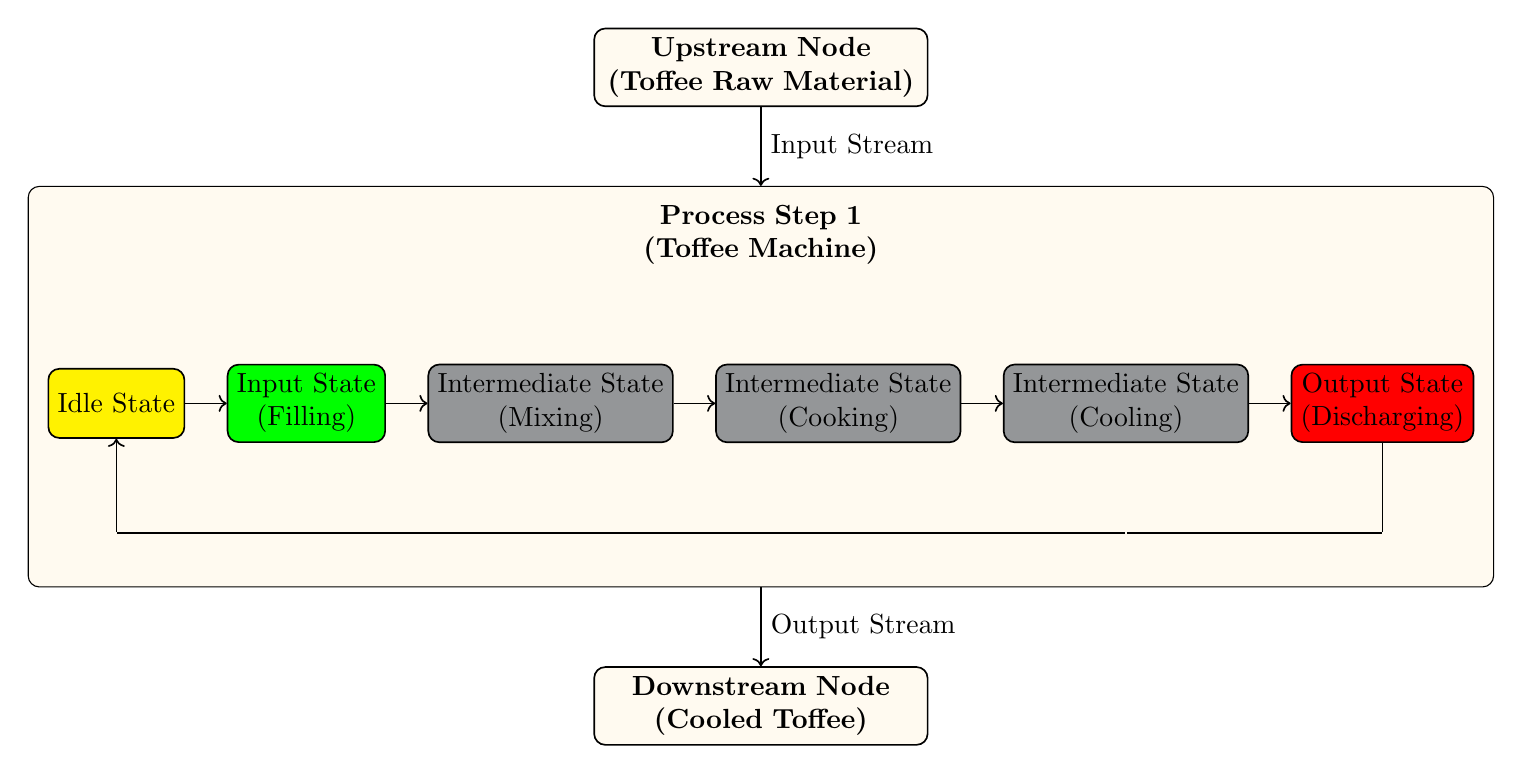
\begin{tikzpicture}[->,auto,node distance=1cm,on grid,semithick]


    \matrix [column sep=15,row sep=20](process_step_matrix)
    {


        % \node[state,rounded corners,rectangle,draw=none](direct_output_at_idle_column){...};                        &
        % \node[state,rounded corners,rectangle,draw=none]{};                                                         &
        % \node[state,rounded corners,rectangle,draw=none]{};                                                         &
        % \node[state,rounded corners,rectangle,draw=none]{};                                                         &
        % \node[state,rounded corners,rectangle,draw=none]{};                                                         &
        % \node[state,rounded corners,rectangle,draw=none]{};                                                         &
        % \node[intermediate_state](direct_pre_output_state){Pre Output State};                                       &   \\



        \node[state,rounded corners,rectangle,style={fill=yellow}](idle_process_state){Idle State};                    &
        \node[state,rounded corners,rectangle,style={fill=green},align=center](input_state){Input State\\ (Filling)}; &
        \node[intermediate_state,align=center](mixing_state){Intermediate State\\ (Mixing)};                                      &
        \node[intermediate_state,align=center](cooking_state){Intermediate State\\(Cooking)};                                     &
        \node[intermediate_state,align=center](cooling_state){Intermediate State\\ (Cooling)};                                    &
        \node[state,rounded corners,rectangle,style={fill=red},align=center](output_state){Output State\\ (Discharging)}; \\

        \node[state,rounded corners,circle,draw=none,inner sep=0pt,minimum size=0pt](first_idle_connection_node){};               &
        \node[state,rounded corners,rectangle,draw=none]{};                                                                       &
        \node[state,rounded corners,rectangle,draw=none]{};                                                                       &
        \node[state,rounded corners,rectangle,draw=none]{};                                                                       &
        \node[state,rounded corners,rectangle,draw=none,inner sep=0pt,minimum size=0pt](pre_idle_state){};                        &
        \node[state,rounded corners,rectangle,draw=none,inner sep=0pt,minimum size=0pt](between_output_and_preidle_state){};            \\
    };

    % % Direct Idle to Output connections
    % \draw (idle_process_state) to (direct_output_at_idle_column);
    % \draw (direct_output_at_idle_column) to (direct_pre_output_state);
    % \draw (direct_pre_output_state) to (output_state);

    % % Input recycle
    % \path (input_state) edge [loop above] node {} (input_state);
    % \draw (input_state) to (pre_input_stream_state);
    % \draw (input_state) to [bend right](between_idle_and_input);

    % \node[draw,path_1_highlighter,fit=(idle_process_state),rect={dashed}{dashed}{dashed}{}]{};

    % % (pre_idle_state)

    % \path let \p1 =(first_idle_connection_node) in
    % node[state,rounded corners,rectangle,draw=none,text opacity=0] (SubIdleMockState) at (\p1) {Idle State};
    % \path let \p1 =(between_output_and_preidle_state) in
    % node[state,rounded corners,rectangle,draw=none,text opacity=0] (SubOutputStateMock) at (\p1) {Pre Output State};
    % \path let \p1 =(output_state) in
    % node[state,rounded corners,rectangle,draw=none,text opacity=0] (OutputStateMock) at (\p1) {Pre Output State};
    % \path let \p1 =(direct_output_at_idle_column) in
    % node[state,rounded corners,rectangle,draw=none,text opacity=0] (AboveIdleMockState) at (\p1) {Idle State};




    % % Idle to Output over input state
    \draw (idle_process_state) to (input_state);
    \draw (input_state) to (mixing_state);
    \draw (mixing_state) to (cooking_state);
    \draw (cooking_state) to (cooling_state);
    \draw (cooling_state) to (output_state);
    % \draw (between_idle_and_input) to (pre_input_stream_state);
    % \draw (pre_input_stream_state) to (input_state);
    % \draw (input_state) to (between_input_and_preoutput_state);
    % \draw (input_state) to (between_input_and_preoutput_state);
    % \draw (between_input_and_preoutput_state) to (preoutput_state);
    % \draw (preoutput_state) to (output_state);

    %Output to idle
    \draw[-] (output_state) to (between_output_and_preidle_state);
    \draw[-] (between_output_and_preidle_state) to (pre_idle_state);
    \draw[-] (pre_idle_state) to (first_idle_connection_node);
    \draw (first_idle_connection_node) to (idle_process_state);




    % Frame and label for process step
    \node[align=center,text width=3 cm,above= of process_step_matrix.north](test){\textbf{Process Step 1 (Toffee Machine)}};
    \begin{scope}[on background layer]
        \node[draw,fit=(test)(process_step_matrix),process_step_node](process_step_outer_frame){};
    \end{scope}
    % Upstream and downstream nodes and connections    
    \node[draw,above= of process_step_outer_frame.north,process_step_node,align=center,text width=4 cm] (upstream_process_step){\textbf{Upstream Node (Toffee Raw Material) }};
    \node[draw,below= of process_step_outer_frame.south,process_step_node,align=center,text width=4 cm] (downstream_process_step){\textbf{Downstream Node (Cooled Toffee)}};
    \draw (upstream_process_step) --  (process_step_outer_frame) node[midway]{Input Stream};
    \draw (process_step_outer_frame) -- (downstream_process_step) node[midway]{Output Stream};







\end{tikzpicture}
\end{document}
